\chapter{Introducción}

Este trabajo de fin de máster es una continuación del trabajo de fin de grado que realicé en el que se desarrolló un \textit{software} (3DCurator) para visualizar un conjunto de datos volumétricos, en formato DICOM, de esculturas de madera policromada.

Con este \textit{software}, los expertos en la materia como restauradores o historiadores del arte podían inspeccionar el interior de las esculturas sin dañarlas para un posterior proceso de estudio, restauración y/o conservación.

En este trabajo de fin de máster se llevarán a cabo distintas tareas de desarrollo que se integrarán a 3DCurator así como un estudio teórico más completo del proceso de obtención de datos volumétricos en los objetos que abarcan el campo de estudio en cuestión.

Las tareas de desarrollo que se integrarán con el \textit{software} desarrollado se dividen en tres bloques:

\begin{itemize}
	\item \textbf{Pre-procesamiento de datos}: Se estudiarán los distintos filtros disponibles para ver cuáles ofrecen mejores resultados en la tarea de reducción de ruido.
	\item \textbf{Subdivisión de piezas de madera}: Las esculturas suelen estar formadas por distintas piezas de madera. Se estudiará la forma de segmentarla probando, en primer lugar, los algoritmos ya existentes utilizados principalmente en medicina. Si ninguno ofrece los resultados que esperamos, se pasará a desarrollar uno propio.
	\item \textbf{Herramientas de documentación}: Se incluirán herramientas para ayudar a los usuarios en la tarea de documentación permitiendo, por ejemplo, incluir distintas anotaciones en puntos de interés.
\end{itemize}

Además de las librerías que ya se utilizaron: VTK \cite{vtk} (visualización), Qt \cite{qt} (GUI) y Boost \cite{boost} (XML); se utilizarán las librerías ITK \cite{itk} y OpenCV \cite{opencv} para el análisis de imágenes y la visión por computador respectivamente. Haciendo uso de CMake \cite{cmake} para pre-compilarlas todas juntas.

Antes de empezar a profundizar en aspectos técnicos se realizará una introducción al proceso de obtención de datos volumétricos usando una Tomografía Computarizada así como de los objetos que se quieren analizar con esta técnica de obtención de datos: las esculturas de madera policromada.

\section{Tomografía Computarizada}

\subsection{Historia}

La tomografía computarizada (TC) es una técnica de obtención de imágenes muy utilizado en el campo de la medicina para, por ejemplo, localizar y ver el tamaño de tumores.

Sus orígenes se remontan a los años 60 cuando en 1967 Goodfrey Newblod Hounsfield propuso la elaboración del que llamó escáner EMI, base para desarrollar el Tomógrafo Axial Computarizado (TAC). El objetivo era ``\textit{crear una imagen tridimensional de un objeto tomando múltiples mediciones del mismo con la misma fuente de rayos X desde diferentes ángulos y utilizar un ordenador que permita reconstruir a partir de cientos de `planos' superpuestos y entrecruzados}'' \cite{gonzales11}.

Cuatro años más tarde, en 1971, se realizó con éxito el primer escáner cerebral usando este tomógrafo. En 1972 se instaló permanentemente en el hospital donde realizaron las pruebas y al año siguiente ya era solicitado por hospitales alrededor de todo el mundo.

\subsection{Generaciones}

El sistema de tomografía computarizada ha pasado por cuatro generaciones \cite{sarrio16}:

\subsubsection{Primera generación}

La adquisición de datos en la primera generación se basaba en la geometría del haz de rayos X paralelo y traslación-rotación en un tubo de rayos X y un solo detector (Figura \ref{fig:introduccion/primera-generacion}). El haz de rayos X se colimaba en dimensiones de 2 x 13mm. Estos 13mm correspondían al grosor del corte. Se tomaba una medida por cada 160 rotaciones durante 180 traslaciones dando un total de 28.800 medidas. El proceso era lento, tardaba unos 5 minutos, y el movimiento del paciente afectaba muy negativamente a la calidad de la imagen, por lo que su uso se veía reducido al escaneo de zonas que podían mantenerse inmóviles como la cabeza.

\begin{figure}[H]
	\centering
	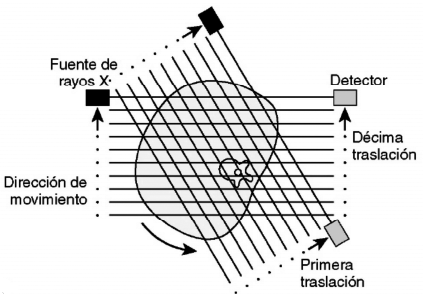
\includegraphics[width=10cm]{imagenes/introduccion/primera-generacion}
	\caption{Primera generación de aparatos de tomografía computarizada \cite{garcia14}}
	\label{fig:introduccion/primera-generacion}
\end{figure}

\subsubsection{Segunda generación}

En esta segunda generación se aumentó el número de detectores (de 5 a 30) por lo que se vio disminuido el tiempo de la exploración a unos 18 segundos (Figura \ref{fig:introduccion/segunda-generacion}).

\begin{figure}[H]
	\centering
	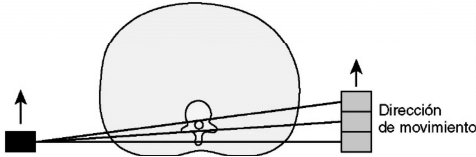
\includegraphics[width=10cm]{imagenes/introduccion/segunda-generacion}
	\caption{Segunda generación de aparatos de tomografía computarizada \cite{garcia14}}
	\label{fig:introduccion/segunda-generacion}
\end{figure}

\subsubsection{Tercera generación}

La tercera generación supuso un gran cambio y se ha convertido en la configuración estándar utilizada en la mayoría de los sistemas de escáner. Se utiliza una geometría de haz en abanico de gran angular (50º a 55º), un arco de detectores y un tubo de rayos X. Estos elementos giran 360º alrededor del paciente (Figura \ref{fig:introduccion/tercera-generacion}). El número de detectores se encuentra entre 600 y 900. Con este sistema el tiempo de barrido oscila entre 3 y 10 segundos.

\begin{figure}[H]
	\centering
	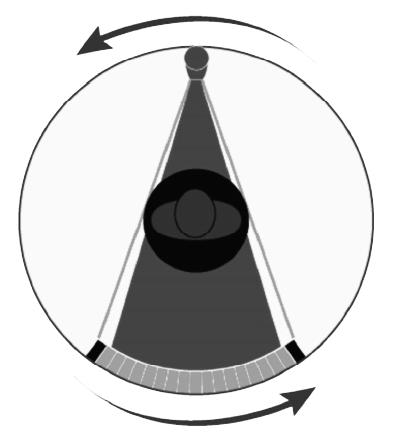
\includegraphics[width=6cm]{imagenes/introduccion/tercera-generacion}
	\caption{Tercera generación de aparatos de tomografía computarizada \cite{garcia14}}
	\label{fig:introduccion/tercera-generacion}
\end{figure}

\subsubsection{Cuarta generación}

La cuarta generación es muy parecida a la tercera solo que añade una configuración de giro estacionario (Figura \ref{fig:introduccion/cuarta-generacion}).

\begin{figure}[H]
	\centering
	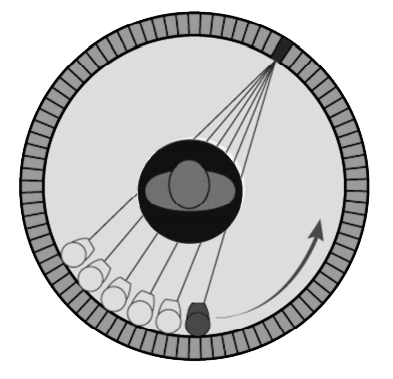
\includegraphics[width=6cm]{imagenes/introduccion/cuarta-generacion}
	\caption{Cuarta generación de aparatos de tomografía computarizada \cite{garcia14}}
	\label{fig:introduccion/cuarta-generacion}
\end{figure}

\subsubsection{Nuevas tecnologías}

\begin{itemize}
	\item \textbf{TC helicoidal (TCH)}: Hasta finales de los años 80, los aparatos de TC adquirían los datos en cortes según un método conocido como exploración axial (de ahí el nombre de TAC). Con los sistemas de tipo helicoidal los datos se obtienen de forma continua mientras se avanza la mesa a través del \textit{gantry} haciendo que el tubo de rayos X describa una trayectoria helicoidal (Figura \ref{fig:introduccion/tch}).
	
	\begin{figure}[H]
		\centering
		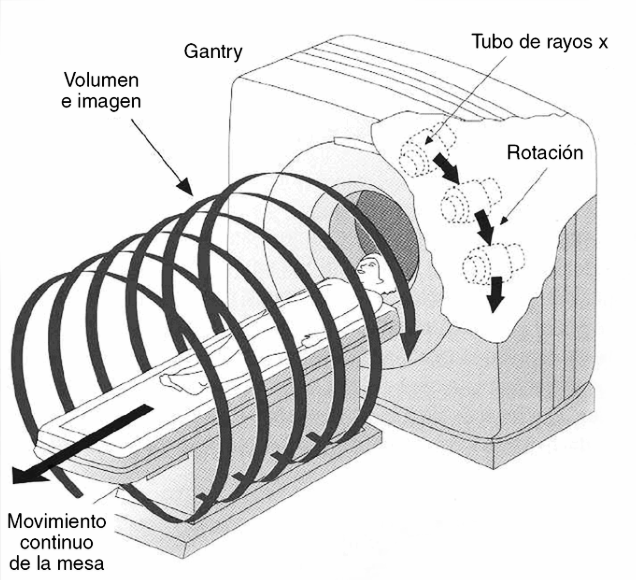
\includegraphics[width=9cm]{imagenes/introduccion/tch}
		\caption{Cuarta generación de aparatos de tomografía computarizada \cite{garcia14}}
		\label{fig:introduccion/tch}
	\end{figure}
	
	\item \textbf{TC helicoidal multicorte (TCM)}: En el lugar donde había una fila de detectores, se colocan múltiples filas. Los primeros tenían 4 filas contiguas, pero posteriormente se ha pasado a alrededor de 16 y 64 filas (Figura \ref{fig:introduccion/tcm}). Por cada rotación se estudia un mayor volumen aumentando así la velocidad de rotación y por tanto los tiempos de exposición obteniendo imágenes de mayor calidad.
	
	\begin{figure}[H]
		\centering
		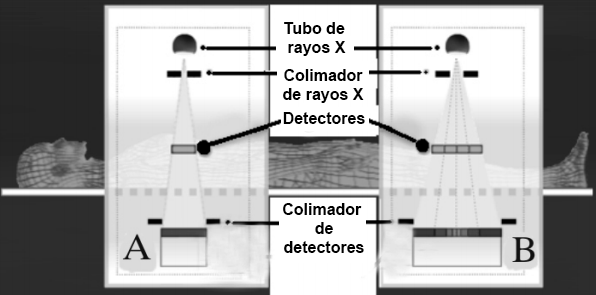
\includegraphics[width=10cm]{imagenes/introduccion/tcm}
		\caption{Diferencias entre TC helicoidal multicorte (B) y monocorte (A) \cite{sarrio16}}
		\label{fig:introduccion/tcm}
	\end{figure}

	\item \textbf{TC de doble fuente (TCED)}: Es uno de los equipos más novedosos pues permiten realizar estudios con diferentes espectros de rayos X. Utilizan dos tubos de rayos X colocados de forma perpendicular en el \textit{gantry} (Figura \ref{fig:introduccion/tced}). Se obtiene por tanto una resolución temporal equivalente a un cuarto del tiempo de rotación del \textit{gantry}.
	
	\begin{figure}[H]
		\centering
		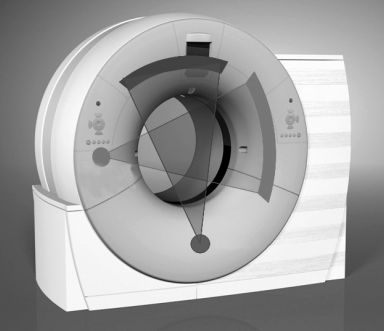
\includegraphics[width=9cm]{imagenes/introduccion/tced}
		\caption{Equipo TC con doble fuente \cite{sarrio16}}
		\label{fig:introduccion/tced}
	\end{figure}

\end{itemize}



\section{Esculturas de madera policromadas}

\subsection{Historia}

El tallado es el método de elaboración de esculturas más antiguo conocido. Se ha tallado en distintos materiales (madera, piedra, marfil...). Pero la madera, por condiciones como su ligereza o la facilidad de ensamblado entre distintas piezas, ha sido uno de los materiales más utilizados.

Se conoce que desde el Antiguo Egipto ya se realizaban esculturas de madera pero es a partir del siglo XI cuando comienza su proliferación. Y desde este momento comienzan a producirse mejoras en las técnicas y herramientas utilizadas durante el proceso del tallado \cite{sarrio16}.

\subsection{Maderas más utilizadas}

Dependiendo del tipo de escultura se utilizan maderas blandas o duras. Si la escultura es más pequeña y contiene más detalles se utilizará un tipo de madera más dura.

No obstante, en la elección también tiene mucha influencia la situación geográfica al utilizarse maderas autóctonas \cite{sarrio16}:

\begin{itemize}
	\item \textbf{Italia}: Álamo y chopo.
	\item \textbf{Francia}: Nogal y castaño.
	\item \textbf{Países Bajos}: Roble y encina.
	\item \textbf{España}: Pino de Flandes, cedro de la Habana, castaño, tejo, álamo, nogal, ciprés, boj, pino silvestre y algunos frutales como el peral.
\end{itemize}

Además de la madera, una escultura de madera policromada, puede contener varios materiales como el estuco o el metal de los clavos utilizados.

\subsection{Defectos de la madera}

Entre los defectos de la madera se pueden encontrar \cite{sarrio16}:

\subsubsection{Grietas o fendas}
Según la UNE-EN 844-9 se denomina grieta o fenda a ``toda separación de las fibras (raja o hendidura) en dirección longitudinal". Según su origen, pueden ser de distintos tipos: 

\begin{itemize}
	\item \textbf{Acebolladuras o \textit{colainas}}: Hay una discontinuidad entre los anillos de crecimiento.
	\item \textbf{Superficiales o de desecación}: Producidas por el calor, provocan un deterioro en las zonas externas del tronco del árbol dejando la madera desprotegida. Provocan grietas en sentido longitudinal.
	\item \textbf{De heladura}: Producidas por una helada dañan la superficie e interior del tronco. Provocan grietas radiales.
	\item \textbf{De viento}: Originadas por la acción de un fuerte viento. Provocan grietas longitudinales y transversales.
\end{itemize}

Además de estos procesos naturales, se pueden producir grietas durante procesos como el secado que provocan una separación de las fibras.

\subsubsection{Fibras reviradas y entrelazadas}

Las fibras se encuentran normalmente orientadas en paralelo al eje principal del tronco, pero en ocasiones pueden presentar nudos que alteran la dirección de éstas.

\subsubsection{Nudos}

La UNE 56.521 define nudo como ``anomalía local de la estructura de la madera producida por la parte inferior de una rama que va quedando englobada en el tronco a medida que se producen los crecimientos de este". Existen distintos tipos:

\begin{itemize}
	\item \textbf{Adherente, vivo, fijo o sano}: Definido por la UNE 56.521 como ``aquel cuyos tejidos son solidarios con los de la madera que los rodea debido a ser formado por una rama viva".
	\item \textbf{Suelto, saltadizo, muerto o seco}: Definido por la UNE 56.521 como ``aquel en que los tejidos de la rama que lo producen no son solidarios con los de la madera que los rodea y suelen separarse".
\end{itemize}

\subsubsection{Núcleos de resina}

Son cavidades entre los anillos de crecimiento producidos frecuentemente por nudos.

\subsubsection{Factores de deterioro de tipo biótico}

Además de las alteraciones que ya presenta la madera, existen otros factores que también influyen como la humedad y la temperatura o el ataque de insectos xilófagos y hongos.

Los insectos xilófagos se nutren de madera seca y favorecen a su desarrollo una humedad relativa y temperaturas no muy bajas. Estos producen daños rompiendo las fibras de la madera.

Los hongos son microorganismos que pueden desarrollarse en la superficie o en el interior de la madera, haciendo que pierda humedad, reduciendo su tamaño y deformándose. Existen tres tipos distintos de degradación tras un ataque de hongos: pudrición blanca, parda o seca y blanda.

\subsection{Proceso de tallado}

El proceso de tallado se podría definir como una técnica sustractiva en la que a partir de una pieza se obtiene una forma concreta.

Un método puede ser utilizar un único bloque de madera. En ocasiones ahuecado por el reverso para contrarrestar fuerza y movimiento de la madera, y, en cierto modo, aligerando el peso.

A partir del siglo XVI empieza a utilizarse con más frecuencia otro método en el que a partir de un bloque principal se ensamblan diferentes piezas generando un bloque más grande, denominado embón, con la forma y el tamaño de la imagen a esculpir. A partir de éste se comienza el tallado.

A partir del Barroco se mejora esta técnica realizando ensamblados en hueco para evitar el posterior ahuecado \cite{sarrio16}.

\section{Estado del arte}

Como ya se ha comentado anteriormente, este trabajo es la continuación del trabajo fin de grado que realicé. Durante este trabajo fin de grado resolví el problema de la visualización de datos volumétricos de esculturas de madera policromada \cite{bolivar16}. Pero no realizaba ningún pre-procesamiento, tan solo se visualizaban permitiendo explorar la escultura en su interior. Toda la información que obtenía el experto que usase el programa debía ser anotada a mano a parte pues tampoco se proporcionaba funcionalidad para almacenar esta información para poder ser rescatada posteriormente.

Este trabajo se divide en tres bloques: pre-procesamiento, documentación y segmentación. 

Los dos primeros están incluidos en la mayoría de los programas disponibles en la web de visualización de datos volumétricos. Tales como AMILab \cite{krissian12}, RadiAnt \cite{radiant}, Slicer \cite{fedorov12} o el usado por María Francisca en su estudio \cite{sarrio16} OsiriX \cite{rosset04} en el que me he inspirado para realizar mi implementación. Todas estas herramientas son muy completas, pero los resultados obtenidos al visualizar los datos volumétricos de esculturas de madera policromadas dejaban mucho que desear y el gran número de funciones específicas para la medicina los hacen complejos de más, y es que por esta razón surgió la idea de crear un software específico de visualización de datos volumétricos de esculturas.

El tercer bloque, el de la segmentación, es totalmente novedoso pues no hay ningún tipo de segmentación específica para separar distintos trozos de madera. Sin embargo, antes de programar un algoritmo específico habría que probar con los que ya hay disponibles que además son muy usados en el campo de la medicina.

Existen varias aproximaciones para llevar a cabo la segmentación en datos volumétricos. Pueden clasificarse en:

\begin{itemize}
	\item Segmentación manual
	\item Segmentación semi-automática
	\item Segmentación basada en umbrales (\textit{thresholding})
	\item Segmentación basada en crecimiento de regiones (\textit{region-growing})
	\item Segmentación basada en bordes (\textit{edge})
\end{itemize}

La segmentación manual la podríamos descartar automáticamente. Pese a que es un método que siempre se puede aplicar, tener a una persona recortando manualmente las distintas piezas corte por corte puede ser muy costoso en cuanto a tiempo.

Los métodos de segmentación basada en umbrales \cite{otsu79} se basan en definir un umbral en los valores escalares de cada vóxel para diferenciar las distintas partes del volumen. Estos no nos son útiles pues las distintas piezas de madera suelen ser del mismo material y coincidir en estos valores de densidad.

Los métodos de segmentación basada en crecimiento de regiones que utilizan umbrales \cite{haralick85} tampoco nos van a servir pues las distintas piezas de madera se encuentran juntas. Otros métodos de segmentación basada en regiones como la transformación divisoria (\textit{watershed}) \cite{beucher79} tampoco nos van a servir pues se definirían muchas cuencas debido a los anillos que presentan los cortes de la madera y si se empiezan a inundar para obtener regiones más grandes obtendremos un resultado similar al que obtenemos con el de crecimiento de regiones con umbrales.

Los métodos de segmentación basados en bordes como el \textit{livewire} \cite{mortensen95} podrían resultar efectivos pues el borde que separa dos piezas de madera es visualmente diferenciable. No obstante, este método necesita de una supervisión humana y, aunque sea más preciso y rápido que una segmentación manual, se debería seguir realizando corte a corte.

Como vemos, ninguno de los métodos que no requieren de supervisión humana son efectivos a la hora de resolver nuestro problema. Es por ello que, definitivamente, hay que desarrollar uno propio.